\section{Launcher}

Um die Profilverwaltung für den Benutzer zu vereinfachen wurde ein Launcher eingeführt. Er hat den Vorteil, dass hier alle letzten Profile angezeigt werden. Auch ist es durch die verbesserte Übersicht, somit für den Benutzer einfacher, Profile zu öffnen oder ein neues Profil zu erstellen.

\begin{figure}[h] 
  \centering
     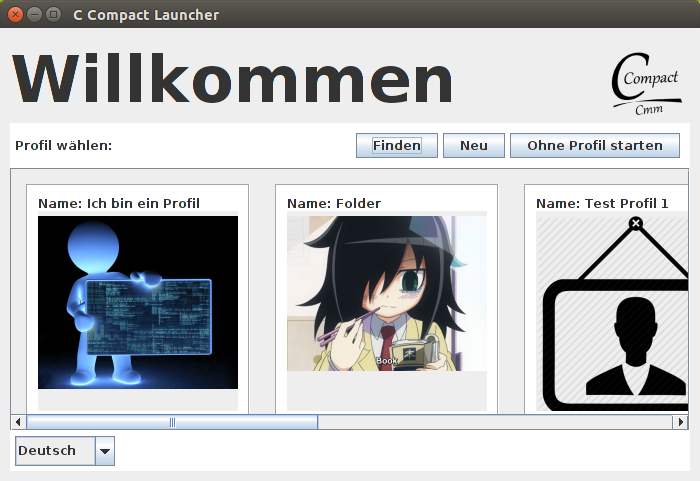
\includegraphics[width=0.9\textwidth]{./media/images/gui/launcher/launcher_main.png}
  \caption{Startbildschirm}
  \label{fig:Bild1}
\end{figure}

Grundsätzlich ist der Launcher ein neues JFrame, das bevor die Benutzeroberfläche gestartet wird angezeigt wird. Die zuletzt verwendeten Profile werden mithilfe einer JScrollpane in welcher sich mehrere JPanels befinden angezeigt. In den JPanels befinden sich der Name und das Benutzerbild.

\begin{itemize}
\item Falls kein Profil angelegt wird, wird auf die Erstellung eines neuen Profils hingewiesen.
\item Wenn der Benutzer kein Profilbild gewählt hat, wird ein voreingestelltes Profilbild verwendet.
\item Mit einem Klick auf das Profilbild kann das gewünschte Profil gestartet werden.
\item Es besteht die Möglichkeit C-Compact mithilfe des Launchers ohne Profil zu starten. Somit ist das Quest-System deaktiviert und es kann nur die normale Entwicklungsumgebung verwendet werden.
\end{itemize}

\subsection{Erstellen eines neuen Profils}
Durch einen Klick auf den Button “Neu”, gelangt man in ein neues Fenster in dem man sein Profil erstellen kann.  

Zuerst wird der Ordnerpfad mithilfe eines JFileChoosers [Kapitel: \ref{sec:JFileChooser}] abgefragt. Falls ein korrekter Pfad ausgewählt wurde, kann nun mithilfe einer JOptionPane ein gewünschter Nutzername gewählt werden. 
\begin{lstlisting}[language=JAVA]
String name = JOptionPane.showInputDialog(null,
"Bitte Namen eingeben?",
 " Eingabeaufforderung",JOptionPane.PLAIN_MESSAGE);
p.setName(name);
\end{lstlisting}

Wenn die Eingabe erfolgreich nicht null ergeben hat, wird nun im gewählten Pfad wird nun ein neuer Ordner erstellt, welcher das Profil mit dem gewählten Namen repräsentiert. Sobald die Einstellungen vorgenommen wurden, wird die Entwicklungsumgebung mit dem neu gestarteten Profil gestartet.

Falls bei der Erstellung des Profils etwas schief läuft oder kein Abgebrochen wird, kommt man automatisch nach anzeigen einer Fehlermeldung wieder zurück zum Launcher.

\subsection{Finden eines bereits existierenden Profils}
Damit ein Profil gestartet werden kann, welches nicht in den letzten Profilen im Launcher vorhanden ist ist es notwendig bereits existierende Profile finden zu lassen.

Sobald man auf den Button “finden”, klickt wird ein veränderter JFileChooser geöffnet. Es können hier nur eine “.cp” Datei ausgewählt werden. Sobald diese angeklickt wurde, wird das Profilbild als Vorschau auf der rechten Seite angezeigt.
